
\begin{figure*}
\centering
\subfloat[Initial configuration - Every nodes get the content from node $R$\label{fig:partition_intuitionA}]{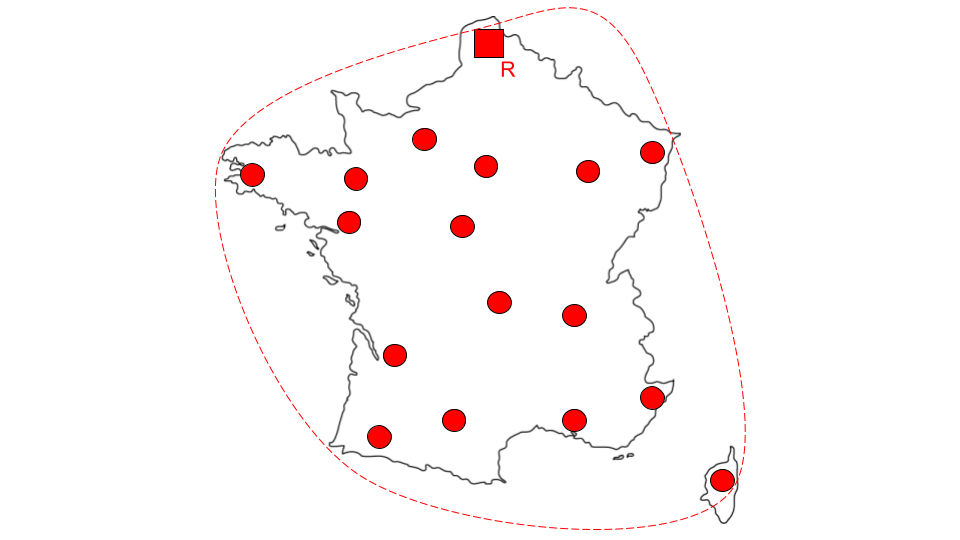
\includegraphics[trim=6cm 0.33cm 6cm 0.33cm, clip, width=0.24\textwidth]{img/Dynamic-partitioning-1.png}}\hfill
\subfloat[Adding a second replica in node $G$ partitions the network nodes in $2$ sets.\label{fig:partition_intuitionB}]{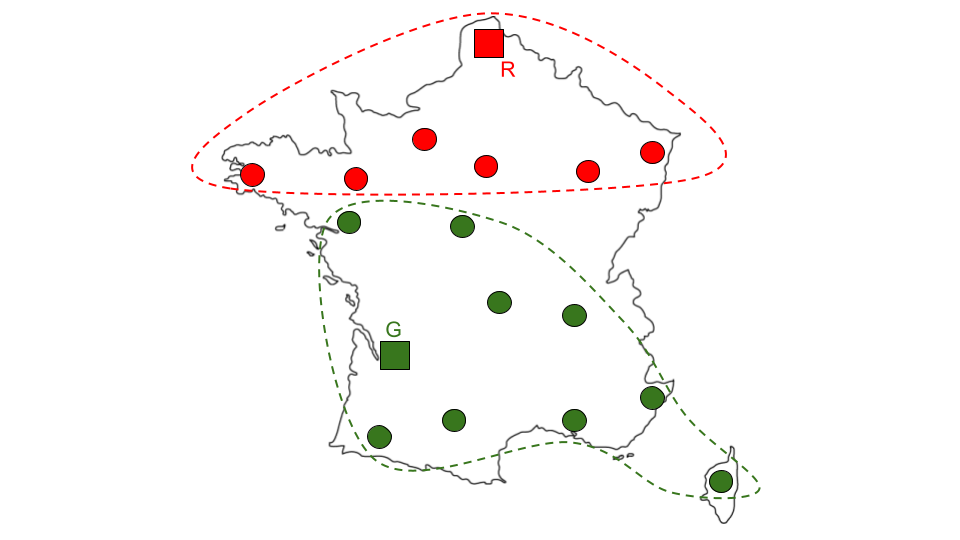
\includegraphics[trim=6cm 0.33cm 6cm 0.33cm, clip, width=0.24\textwidth]{img/Dynamic-partitioning-2.png}}\hfill
\subfloat[A third replica is created in node $B$ resulting in $3$ partitions.\label{fig:partition_intuitionC}]{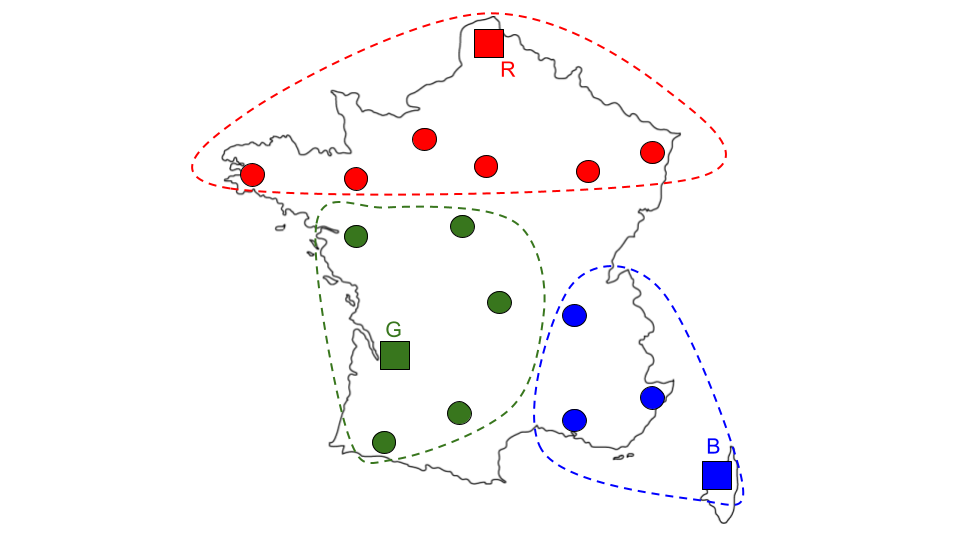
\includegraphics[trim=6cm 0.33cm 6cm 0.33cm, clip, width=0.24\textwidth]{img/Dynamic-partitioning-3.png}}\hfill
\subfloat[Removing the green partition: only $2$ partitions remain.\label{fig:partition_intuitionD}]{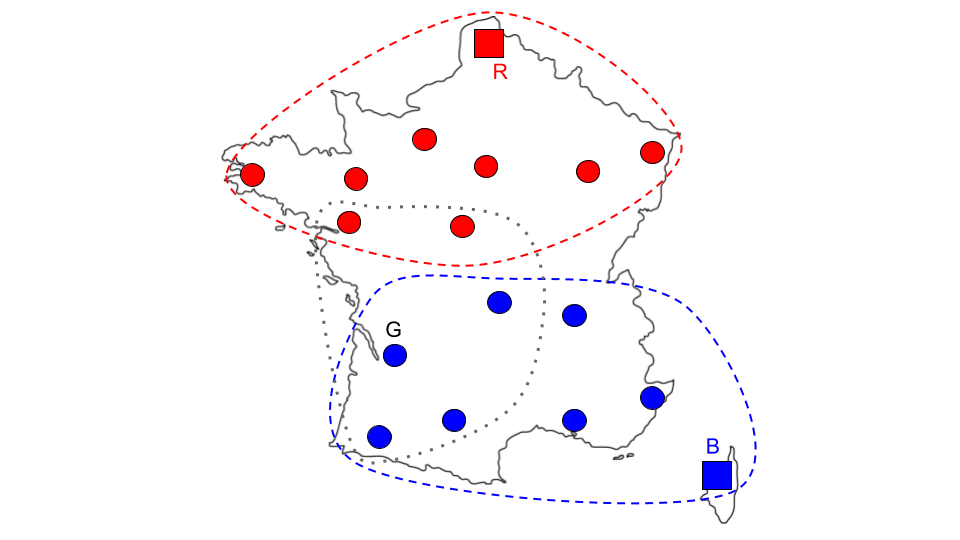
\includegraphics[trim=6cm 0.33cm 6cm 0.33cm, clip, width=0.24\textwidth]{img/Dynamic-partitioning-4.png}}
%
\caption{Example of the french RENATER topology (edges are not drawn):
  Partitions shrink or expand according to the creation or removal of
  replicas. Ideally, only a subset of nodes should be informed of
  these events, according to their place in the
  topology.} \label{fig:partition_intuition}
\end{figure*}

%%% Local Variables: 
%%% mode: latex
%%% TeX-master: "../paper"
%%% ispell-local-dictionary: "english"
%%% End: 
